\section{Qualitative Results}

Figure~\ref{fig:qualitative-results} was generated by loading all four restored best checkpoints and evaluating the official test set in deterministic order. It includes easy examples, cases where CNN and GRU recover errors from simpler models, cases where CNN succeeds but GRU fails, and examples missed by all four models.

\begin{figure}[H]
    \centering
    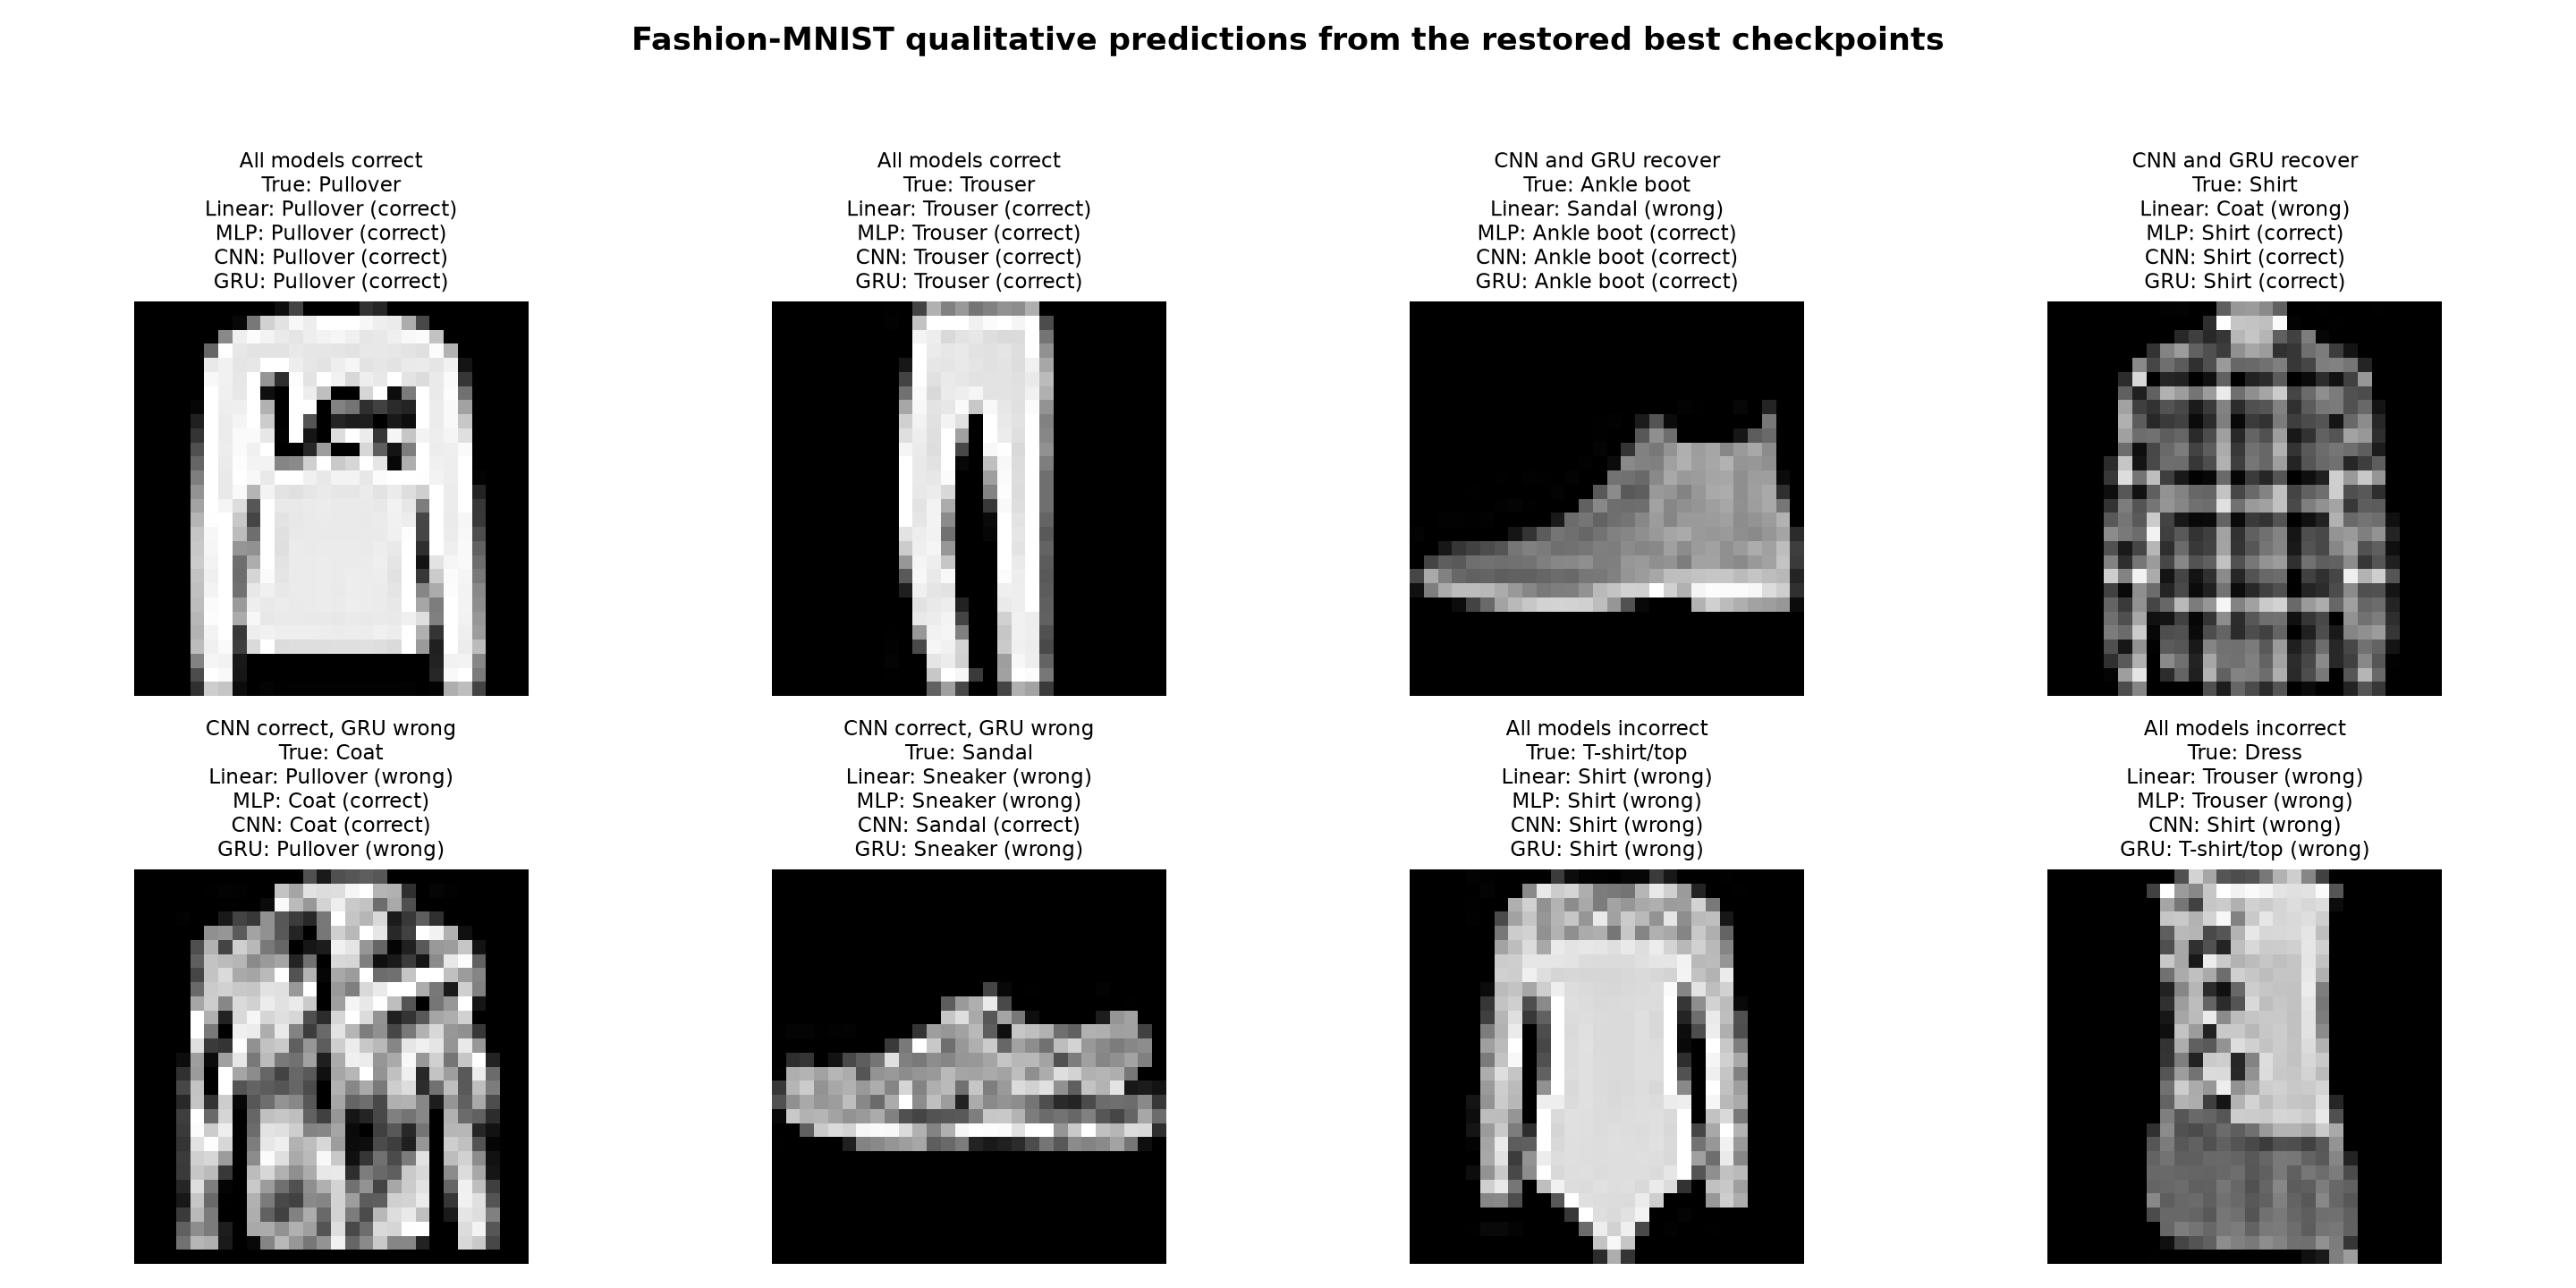
\includegraphics[width=\textwidth]{../../Assignment1/outputs/metrics/qualitative_predictions.png}
    \caption{Correct, difficult-but-correct, and incorrect predictions from Linear, MLP, CNN, and GRU.}
    \label{fig:qualitative-results}
\end{figure}

The examples support three observations. First, distinctive shapes such as Trouser are easy for every representation. Second, structured models recover ambiguous examples that the Linear model misses, including the displayed Ankle boot and Shirt. Third, low-resolution T-shirt/top and Dress examples can remain ambiguous even when CNN and GRU are used; these are genuine failure cases rather than isolated aggregate statistics.

\begin{figure}[H]
    \centering
    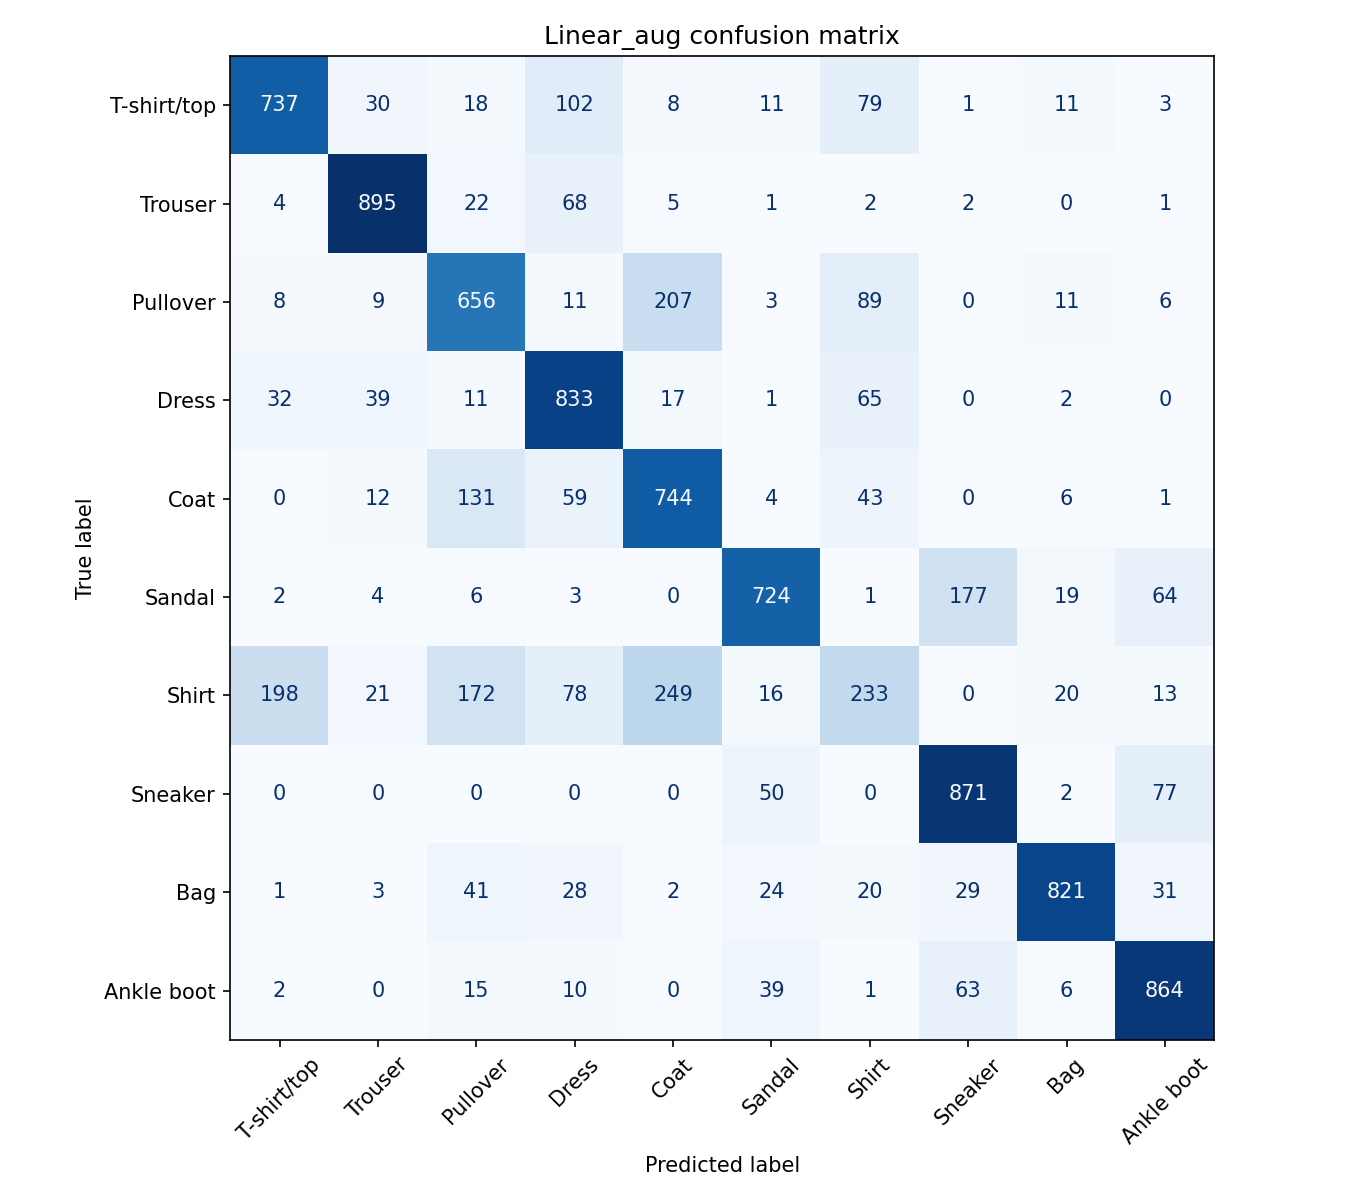
\includegraphics[width=0.48\textwidth]{../../Assignment1/outputs/metrics/linear_aug_confusion_matrix.png}
    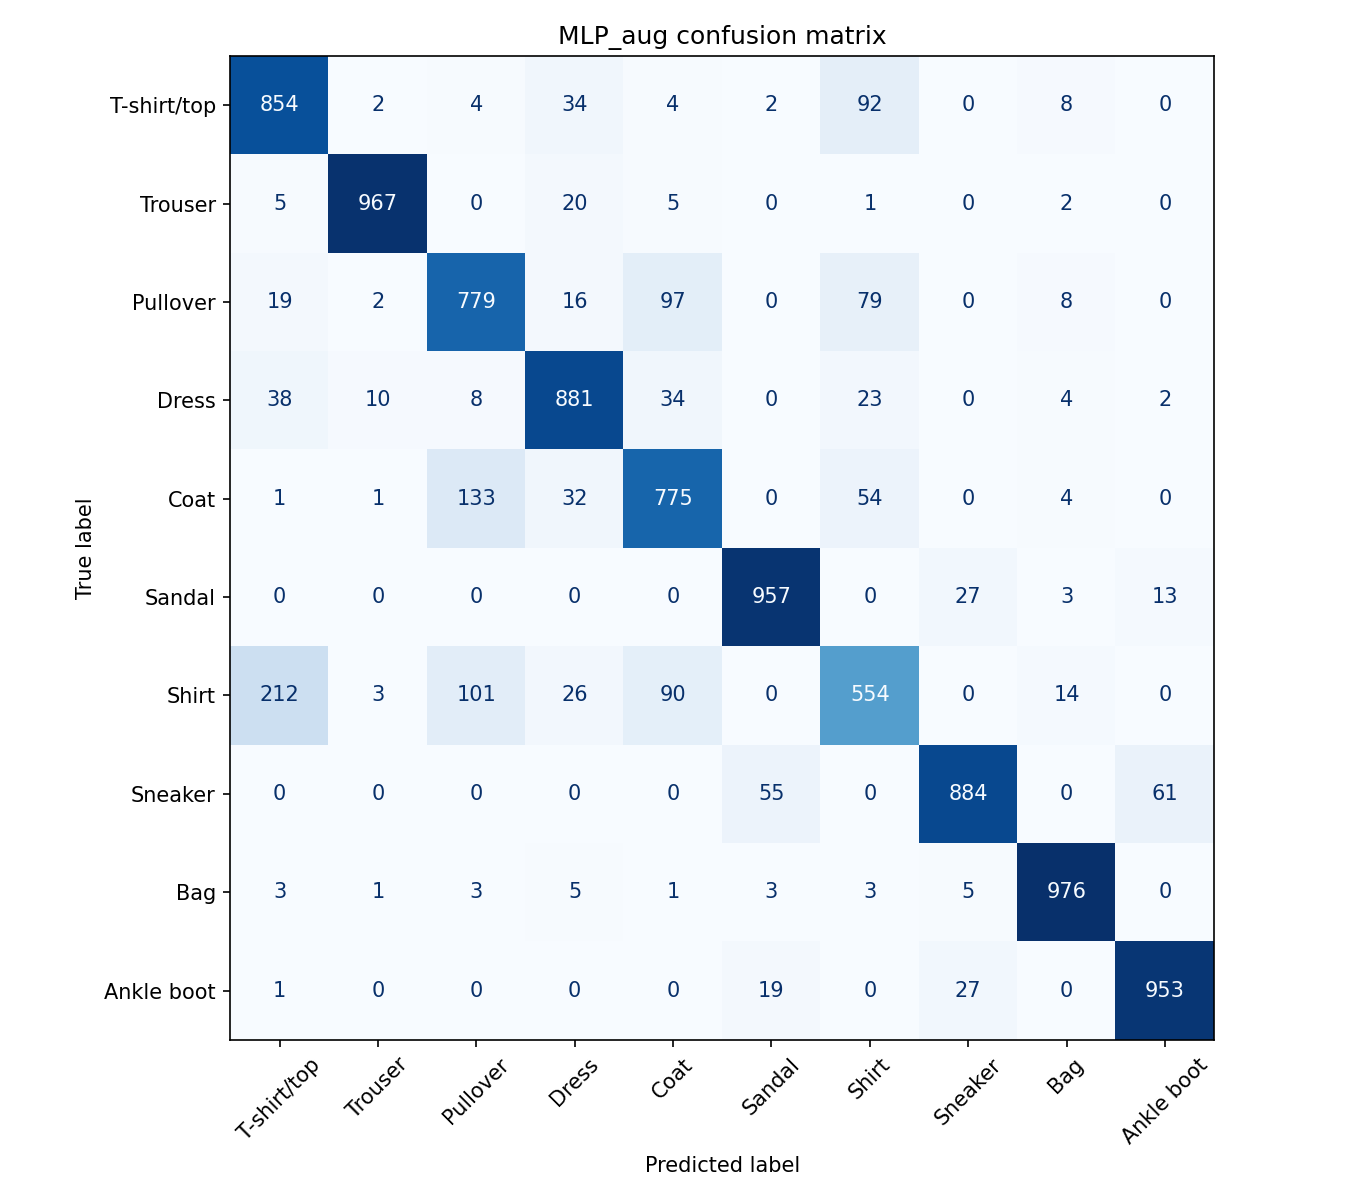
\includegraphics[width=0.48\textwidth]{../../Assignment1/outputs/metrics/mlp_aug_confusion_matrix.png}\\[4pt]
    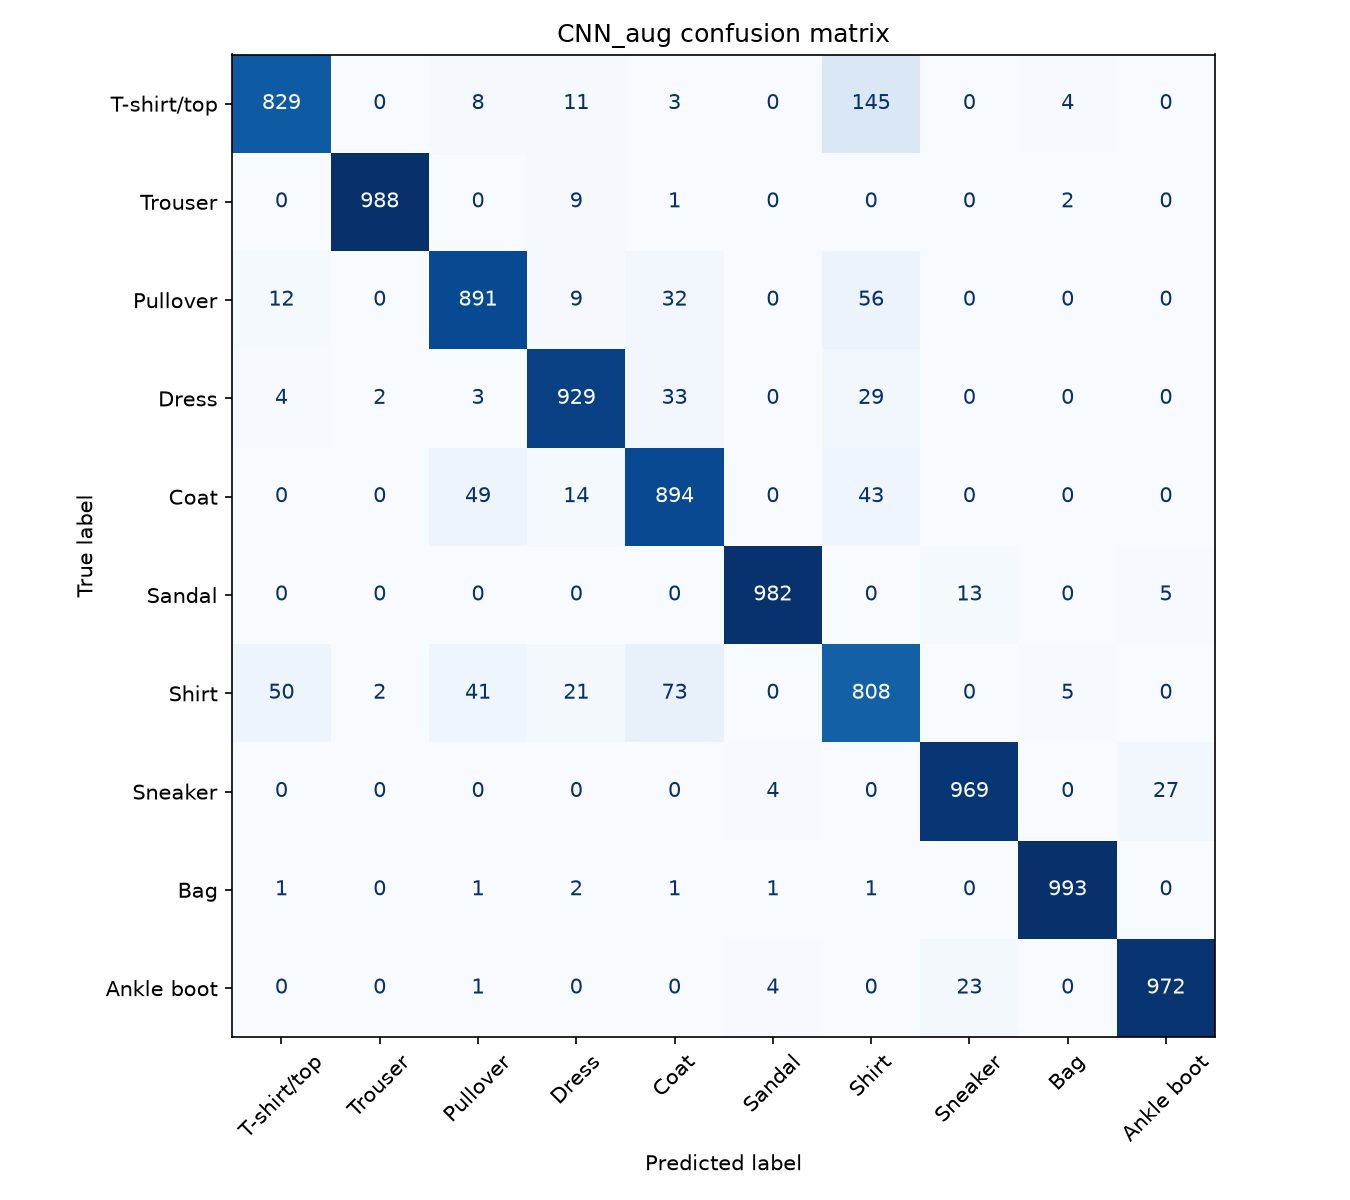
\includegraphics[width=0.48\textwidth]{../../Assignment1/outputs/metrics/cnn_aug_confusion_matrix.png}
    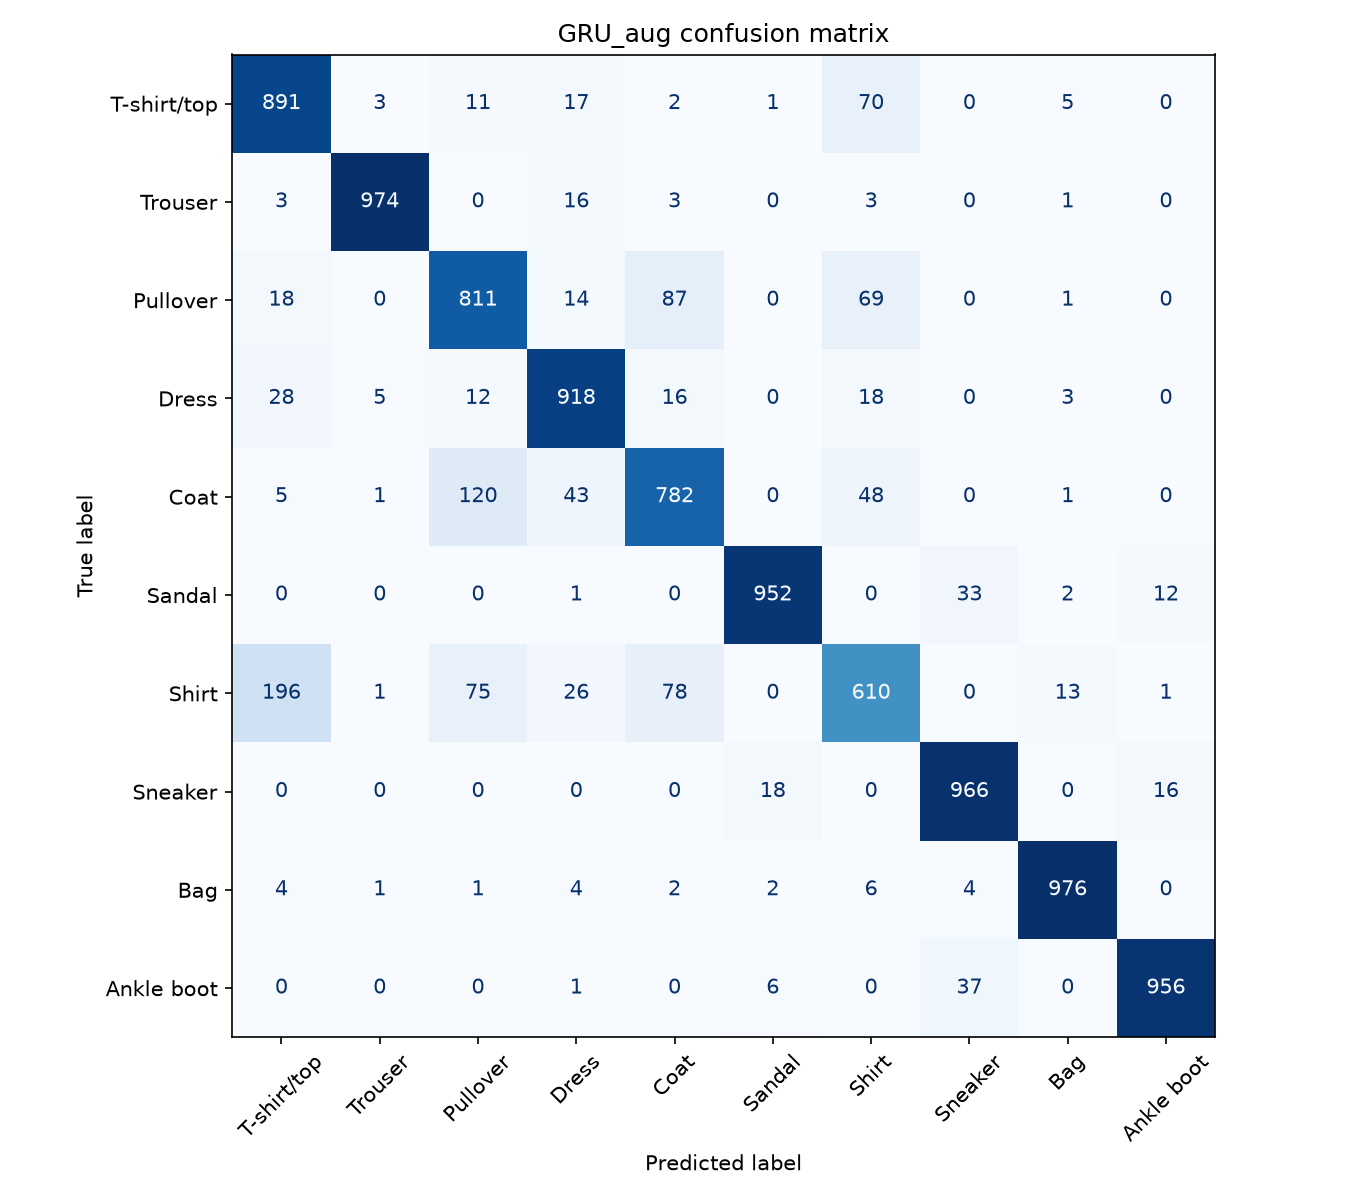
\includegraphics[width=0.48\textwidth]{../../Assignment1/outputs/metrics/gru_aug_confusion_matrix.png}
    \caption{Test confusion matrices in reading order: Linear, MLP, CNN, and GRU.}
    \label{fig:all-confusion-matrices}
\end{figure}
